\section{Evaluation Suite Design}
\label{sec:evaluation-suite}

This section presents a controlled, real-UAV-informed evaluation suite in
AirSim for testing whether CLoMA-UWR remains effective as operational pressure
increases. It instantiates the task model in
Section~\ref{sec:system-design} through real-to-sim calibration, difficulty
stratification, and mission-level metrics, which ground the simulated setting,
vary operational pressure, and separate task completion, execution quality, and
mission continuity. As summarized in Table~\ref{tab:benchmark_comparison},
existing settings cover only parts of the transition from aerial observation to
task-zone construction, resource-constrained mission planning, and runtime
replanning; the comparison concerns evaluation coverage rather than algorithmic
performance. The following subsections detail the three design elements.

% Required packages:
% \usepackage{booktabs}
% \usepackage{makecell}
% \usepackage{graphicx}

% Monochrome symbols are clearer and more appropriate for print publication.
\newcommand{\cmark}{\ensuremath{\bullet}}
\newcommand{\pmark}{\ensuremath{\circ}}
\newcommand{\xmark}{\textemdash}

\begin{table}[!t]
\centering
\caption{Coverage of evaluation capabilities in existing datasets, benchmarks,
and the evaluation suite used in this work.
\cmark indicates explicit coverage, \pmark indicates partial coverage, and \xmark indicates no explicit coverage.}
\label{tab:benchmark_comparison}
\footnotesize
\setlength{\tabcolsep}{1.5pt}
\renewcommand{\arraystretch}{1.08}
\begin{tabular}{
    @{}
    >{\raggedright\arraybackslash}p{0.32\columnwidth}
    *{4}{>{\centering\arraybackslash}p{0.14\columnwidth}}
    @{}}
\toprule
\textbf{Benchmark / dataset}
& \textbf{\makecell{Fire\\perc.}}
& \textbf{\makecell{Disaster\\sem.}}
& \textbf{\makecell{UAV\\constr.}}
& \textbf{\makecell{Runtime\\repl.}} \\
\midrule

DOTA~\cite{xia2018dota}
& \cmark & \xmark & \xmark & \xmark \\

VisDrone~\cite{zhu2022visdrone}
& \cmark & \xmark & \xmark & \xmark \\

UAVs-FFDB~\cite{mowla2024uavsffdb}
& \cmark & \cmark & \xmark & \xmark \\

FLAME~\cite{shamsoshoara2021flame}
& \cmark & \cmark & \xmark & \xmark \\

MS-FSDB~\cite{han2024msfsdb}
& \pmark & \cmark & \xmark & \xmark \\

WildFireVQA~\cite{habibpour2026wildfirevqa}
& \cmark & \cmark & \pmark & \xmark \\

RMASBench~\cite{kleiner2013rmasbench}
& \xmark & \cmark & \pmark & \pmark \\

CrisisBench~\cite{alam2021crisisbench}
& \xmark & \cmark & \xmark & \xmark \\

\midrule
\textbf{Our Evaluation Suite}
& \cmark & \cmark & \cmark & \cmark \\

\bottomrule
\end{tabular}
\end{table}


\begin{figure}[!t]
    \centering
    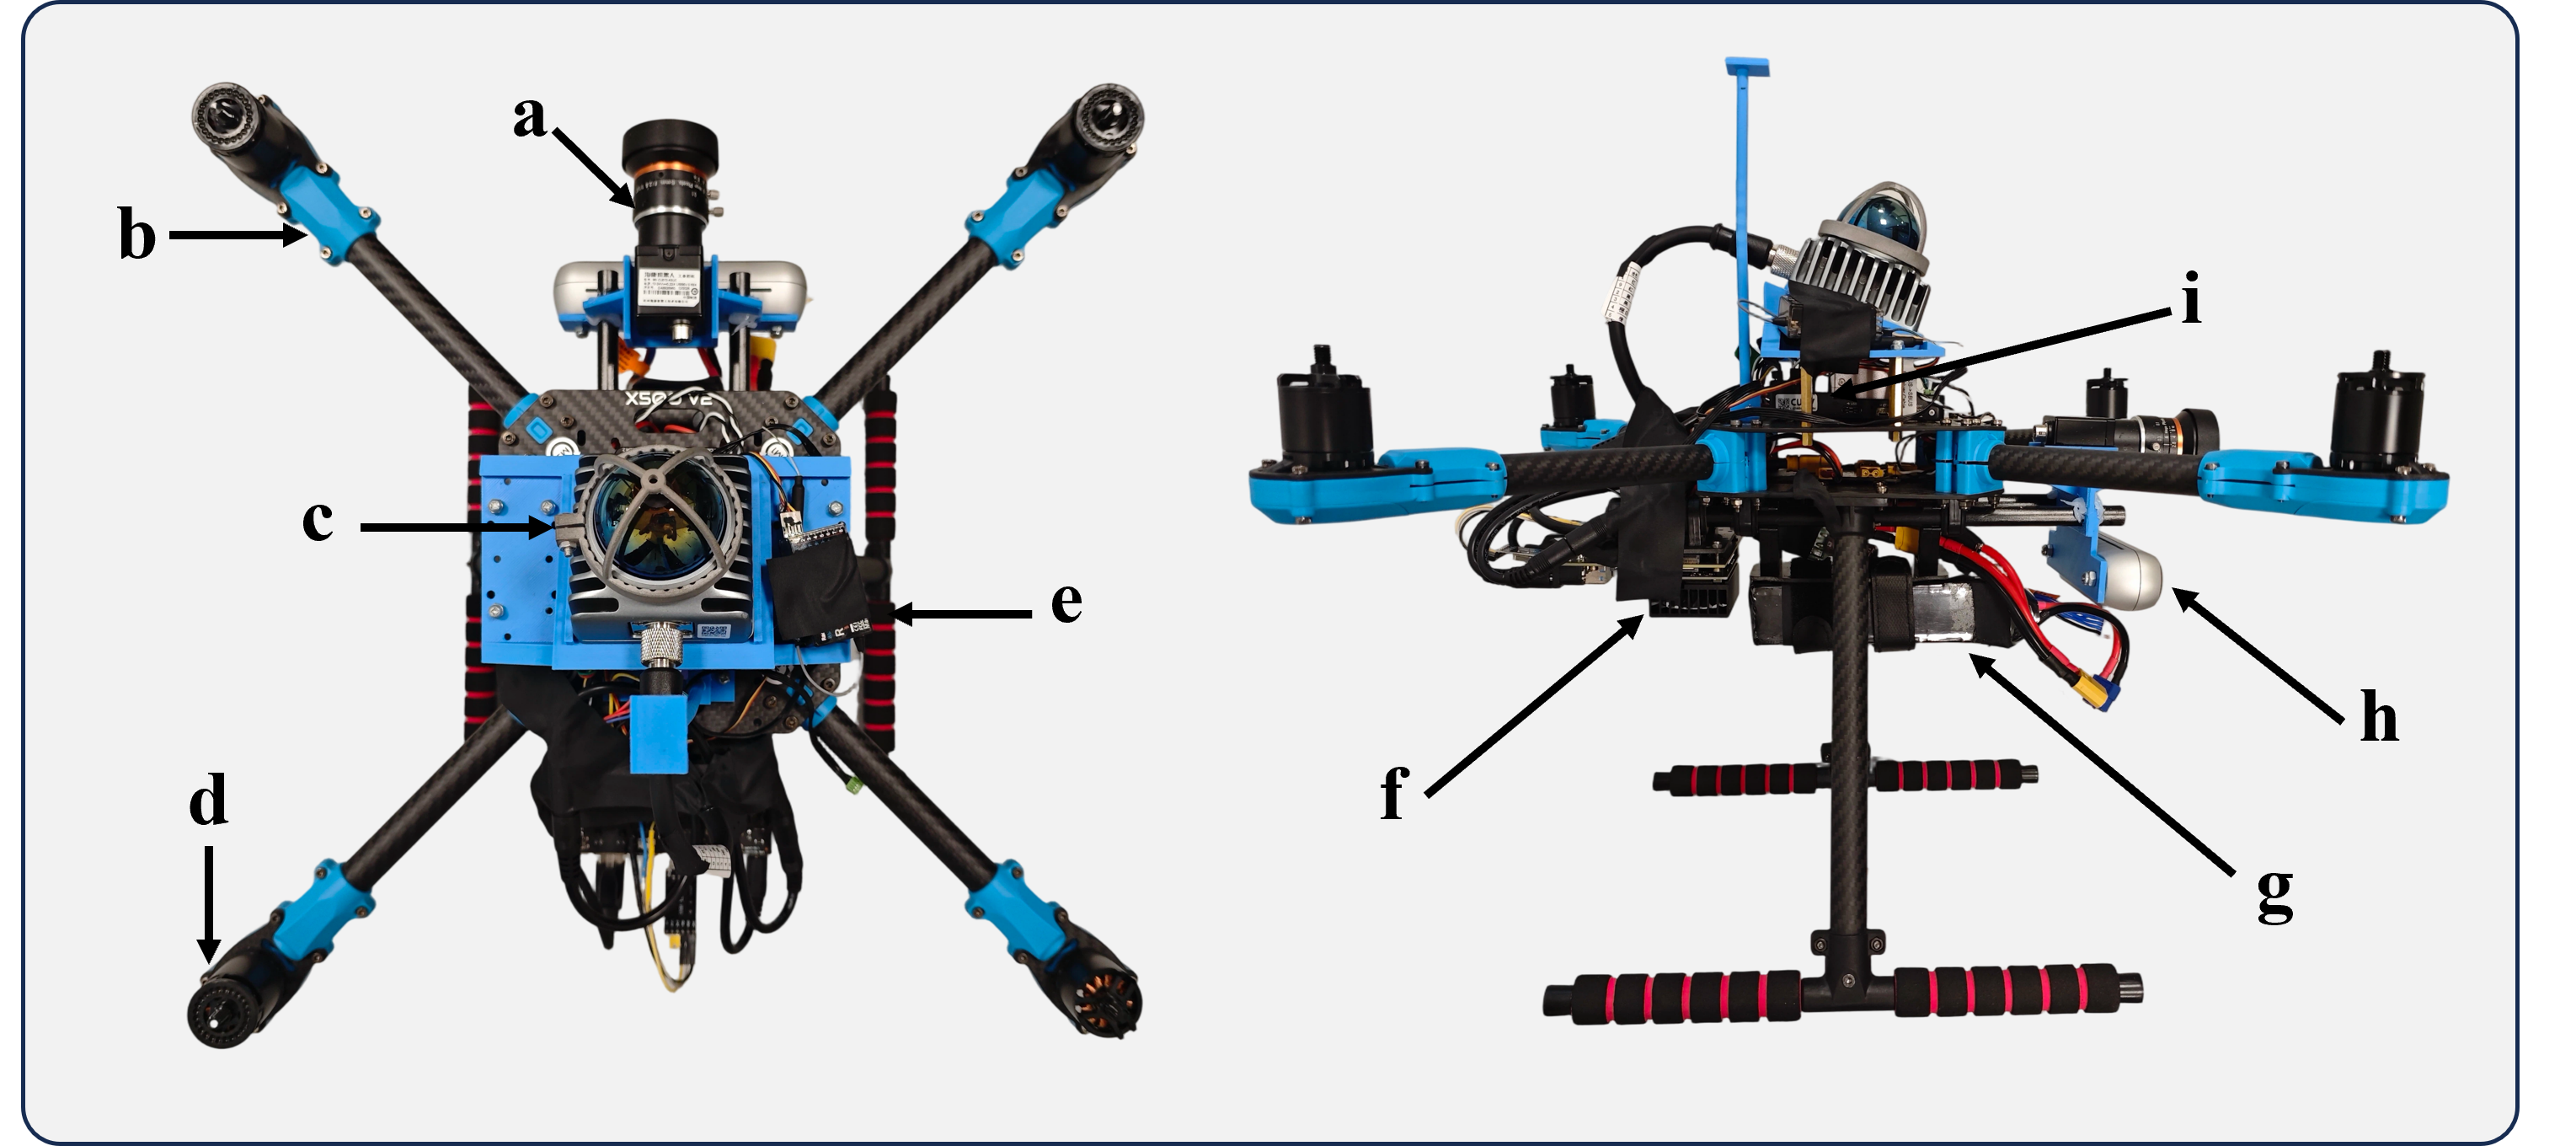
\includegraphics[width=\columnwidth]{figures/real-uav-platform.png}
    \caption{UAV platform and its main components: (a) LiDAR,
    (b) frame, (c) monocular camera, (d) motor, (e) receiver, 
    (f) onboard computer, (g) power supply, 
    (h) stereo camera, and (i) flight controller.}
    \label{fig:UAV-platform}
\end{figure}

\subsection{Real-to-Sim Calibration}
\label{subsec:real-to-sim-calibration}
The first design property is realized through a co-design between the real UAV
platform and the AirSim simulation environment. As stated above, real UAV
parameters constrain every evaluation episode. Accordingly, the real platform defines the
engineering boundary of the rescue mission, while AirSim configures controllable
and repeatable evaluation episodes within that boundary. Rather than treating the two as
separate experimental settings, we use the real platform to define the feasible
set from which AirSim configures each simulated UAV and its environment.
For each UAV, the configured mission must satisfy
\begin{equation}
\begin{aligned}
\mathcal{E}_{\mathrm{UAV}}=\{&(h,v,m,e_{\mathrm{avail}},r)\mid\\
    &h\in \mathcal{H}_{\mathrm{safe}},\quad
      v\in \mathcal{V}_{\mathrm{safe}},\\
    &m\leq m_{\max},\quad
      e_{\mathrm{req}}+e_{\mathrm{res}}\leq e_{\mathrm{avail}},\\
    &r\leq r_{\mathrm{link}}\}.
\end{aligned}
\label{eq:uav-envelope}
\end{equation}
where $\mathcal{E}_{\mathrm{UAV}}$ is the feasible UAV configuration set;
$h$, $v$, $m$, $e_{\mathrm{avail}}$, and $r$ denote flight altitude, velocity,
payload mass, available energy, and communication-link distance,
respectively. $\mathcal{H}_{\mathrm{safe}}$ and
$\mathcal{V}_{\mathrm{safe}}$ are the safe altitude and velocity sets specified
by the operating policy; $m_{\max}$ is the maximum payload mass;
$e_{\mathrm{req}}$ and $e_{\mathrm{res}}$ are the energy required for the
mission and the reserve energy for a safe return; and $r_{\mathrm{link}}$ is the
maximum communication-link distance. These bounds combine hardware
specifications, flight-safety policy, and deployment configuration. Any
configuration that violates
Eq.~\ref{eq:uav-envelope} is excluded before episode generation. The real UAV
platform is shown in Figure~\ref{fig:UAV-platform}, and its hardware
specifications are listed in Table~\ref{tab:real_uav_hardware}.

\input{tables/real-uav-hardware-specifications}

The virtual observation process is further fixed by the real camera geometry.
Under a nadir-view, locally planar-ground approximation, for altitude $h$,
horizontal field of view $\theta_{\mathrm{FOV}}$, and horizontal
resolution $N_x$, the image footprint and ground sampling distance are
\begin{equation}
W(h)=2h\tan\left(\frac{\theta_{\mathrm{FOV}}}{2}\right),\qquad
\mathrm{GSD}(h)=\frac{W(h)}{N_x}.
\label{eq:observation-geometry}
\end{equation}
Thus, the AirSim camera pose and the scale, density, and placement of fire
points are jointly constrained by what the real camera could observe, rather
than selected independently. Energy and payload limits likewise constrain route
length, task duration, and suppressible workload. Table~\ref{tab:real_to_sim_calibration}
records these calibration rules and the resulting simulation settings.

\input{tables/airsim-real-to-sim-calibration}

These calibrated bounds provide the common operational basis on which the
difficulty levels are constructed.

\subsection{Difficulty Stratification}
Each of the four difficulty levels in Table~\ref{tab:scenario-controls}
contains 20 fixed evaluation episodes, yielding 80 episodes in total. The simple
and normal levels test fire-situation understanding and resource-constrained
mission planning without runtime perturbations, whereas the hard and expert
levels introduce progressively stronger resource constraints and scheduling
interactions together with runtime perturbations. All fleet, sensing, energy,
payload, and communication settings
remain within the real-to-sim calibrated bounds in
Section~\ref{subsec:real-to-sim-calibration}.

\input{tables/scenario-difficulty-controls}

The fire-point configurations of all episodes are pre-specified rather than
randomly generated. These configurations control the scene structure
and the spatial arrangement and number of fire points per task zone across
difficulty levels.
Figure~\ref{fig:difficulty-scene-examples} provides representative scenes from
the four difficulty levels, and Figure~\ref{fig:fire-point-count-distribution} summarizes
the distribution of fire-point counts per task zone within each difficulty level. Together,
they illustrate the scene layouts and task-zone-level fire-point distributions
used to instantiate the four difficulty levels.

\begin{figure*}[!t]
    \centering
    \includegraphics[width=1\textwidth]{figures/difficulty-level-fire-scenes.png}
    \caption{Representative fire scenes from the four difficulty levels.
    In each example, \textit{Origin image} denotes the original aerial image,
    and \textit{Perception result} denotes the output generated by the Vision
    Analysis module, which uses Gemini~3.1 Pro as its foundation model.}
    \label{fig:difficulty-scene-examples}
\end{figure*}

\begin{figure}[!t]
    \centering
    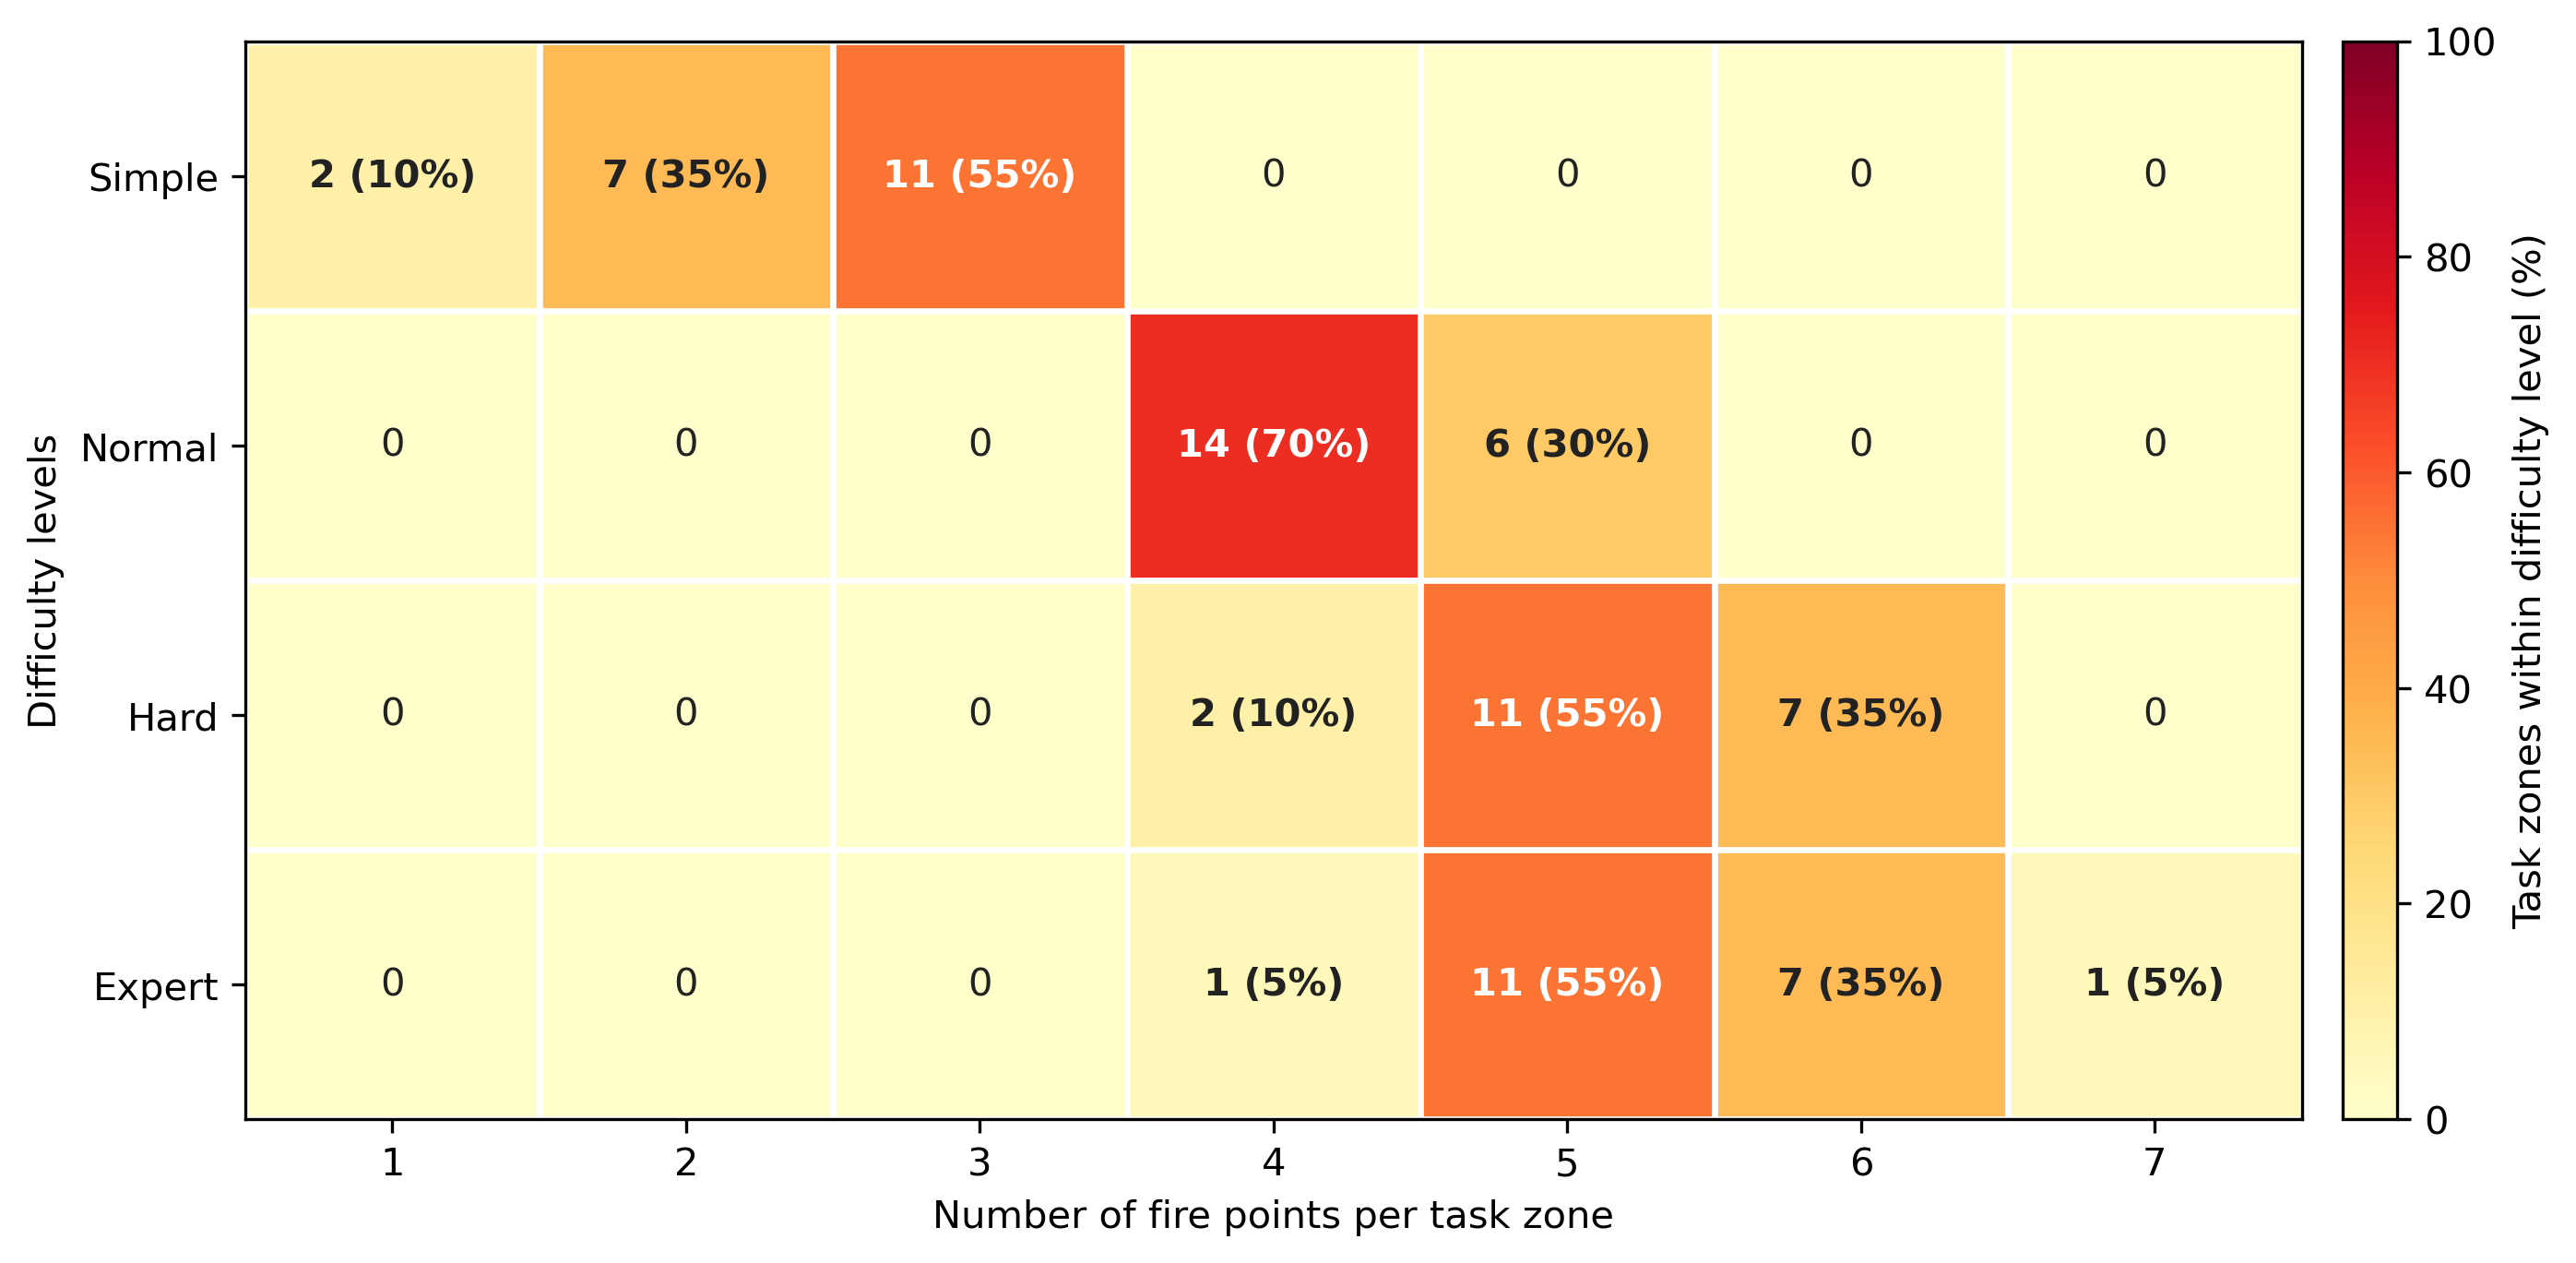
\includegraphics[width=\columnwidth]{figures/task-zone-fire-point-distribution.png}
    \caption{Distribution of fire-point counts per task zone across difficulty
    levels.}
    \label{fig:fire-point-count-distribution}
\end{figure}

Runtime perturbations modify the operational state or mission constraints after
execution begins. Figure~\ref{fig:runtime-perturbation-distribution} summarizes
the five event families and the fixed draws used in hard and expert episodes;
events are sampled once during suite construction and placed at predefined
episode points, with hard episodes using a few temporally separated
perturbations and expert episodes using more frequent, potentially overlapping
perturbations.

\begin{figure*}[!t]
    \centering
    \subfloat[Runtime perturbation library.]{%
        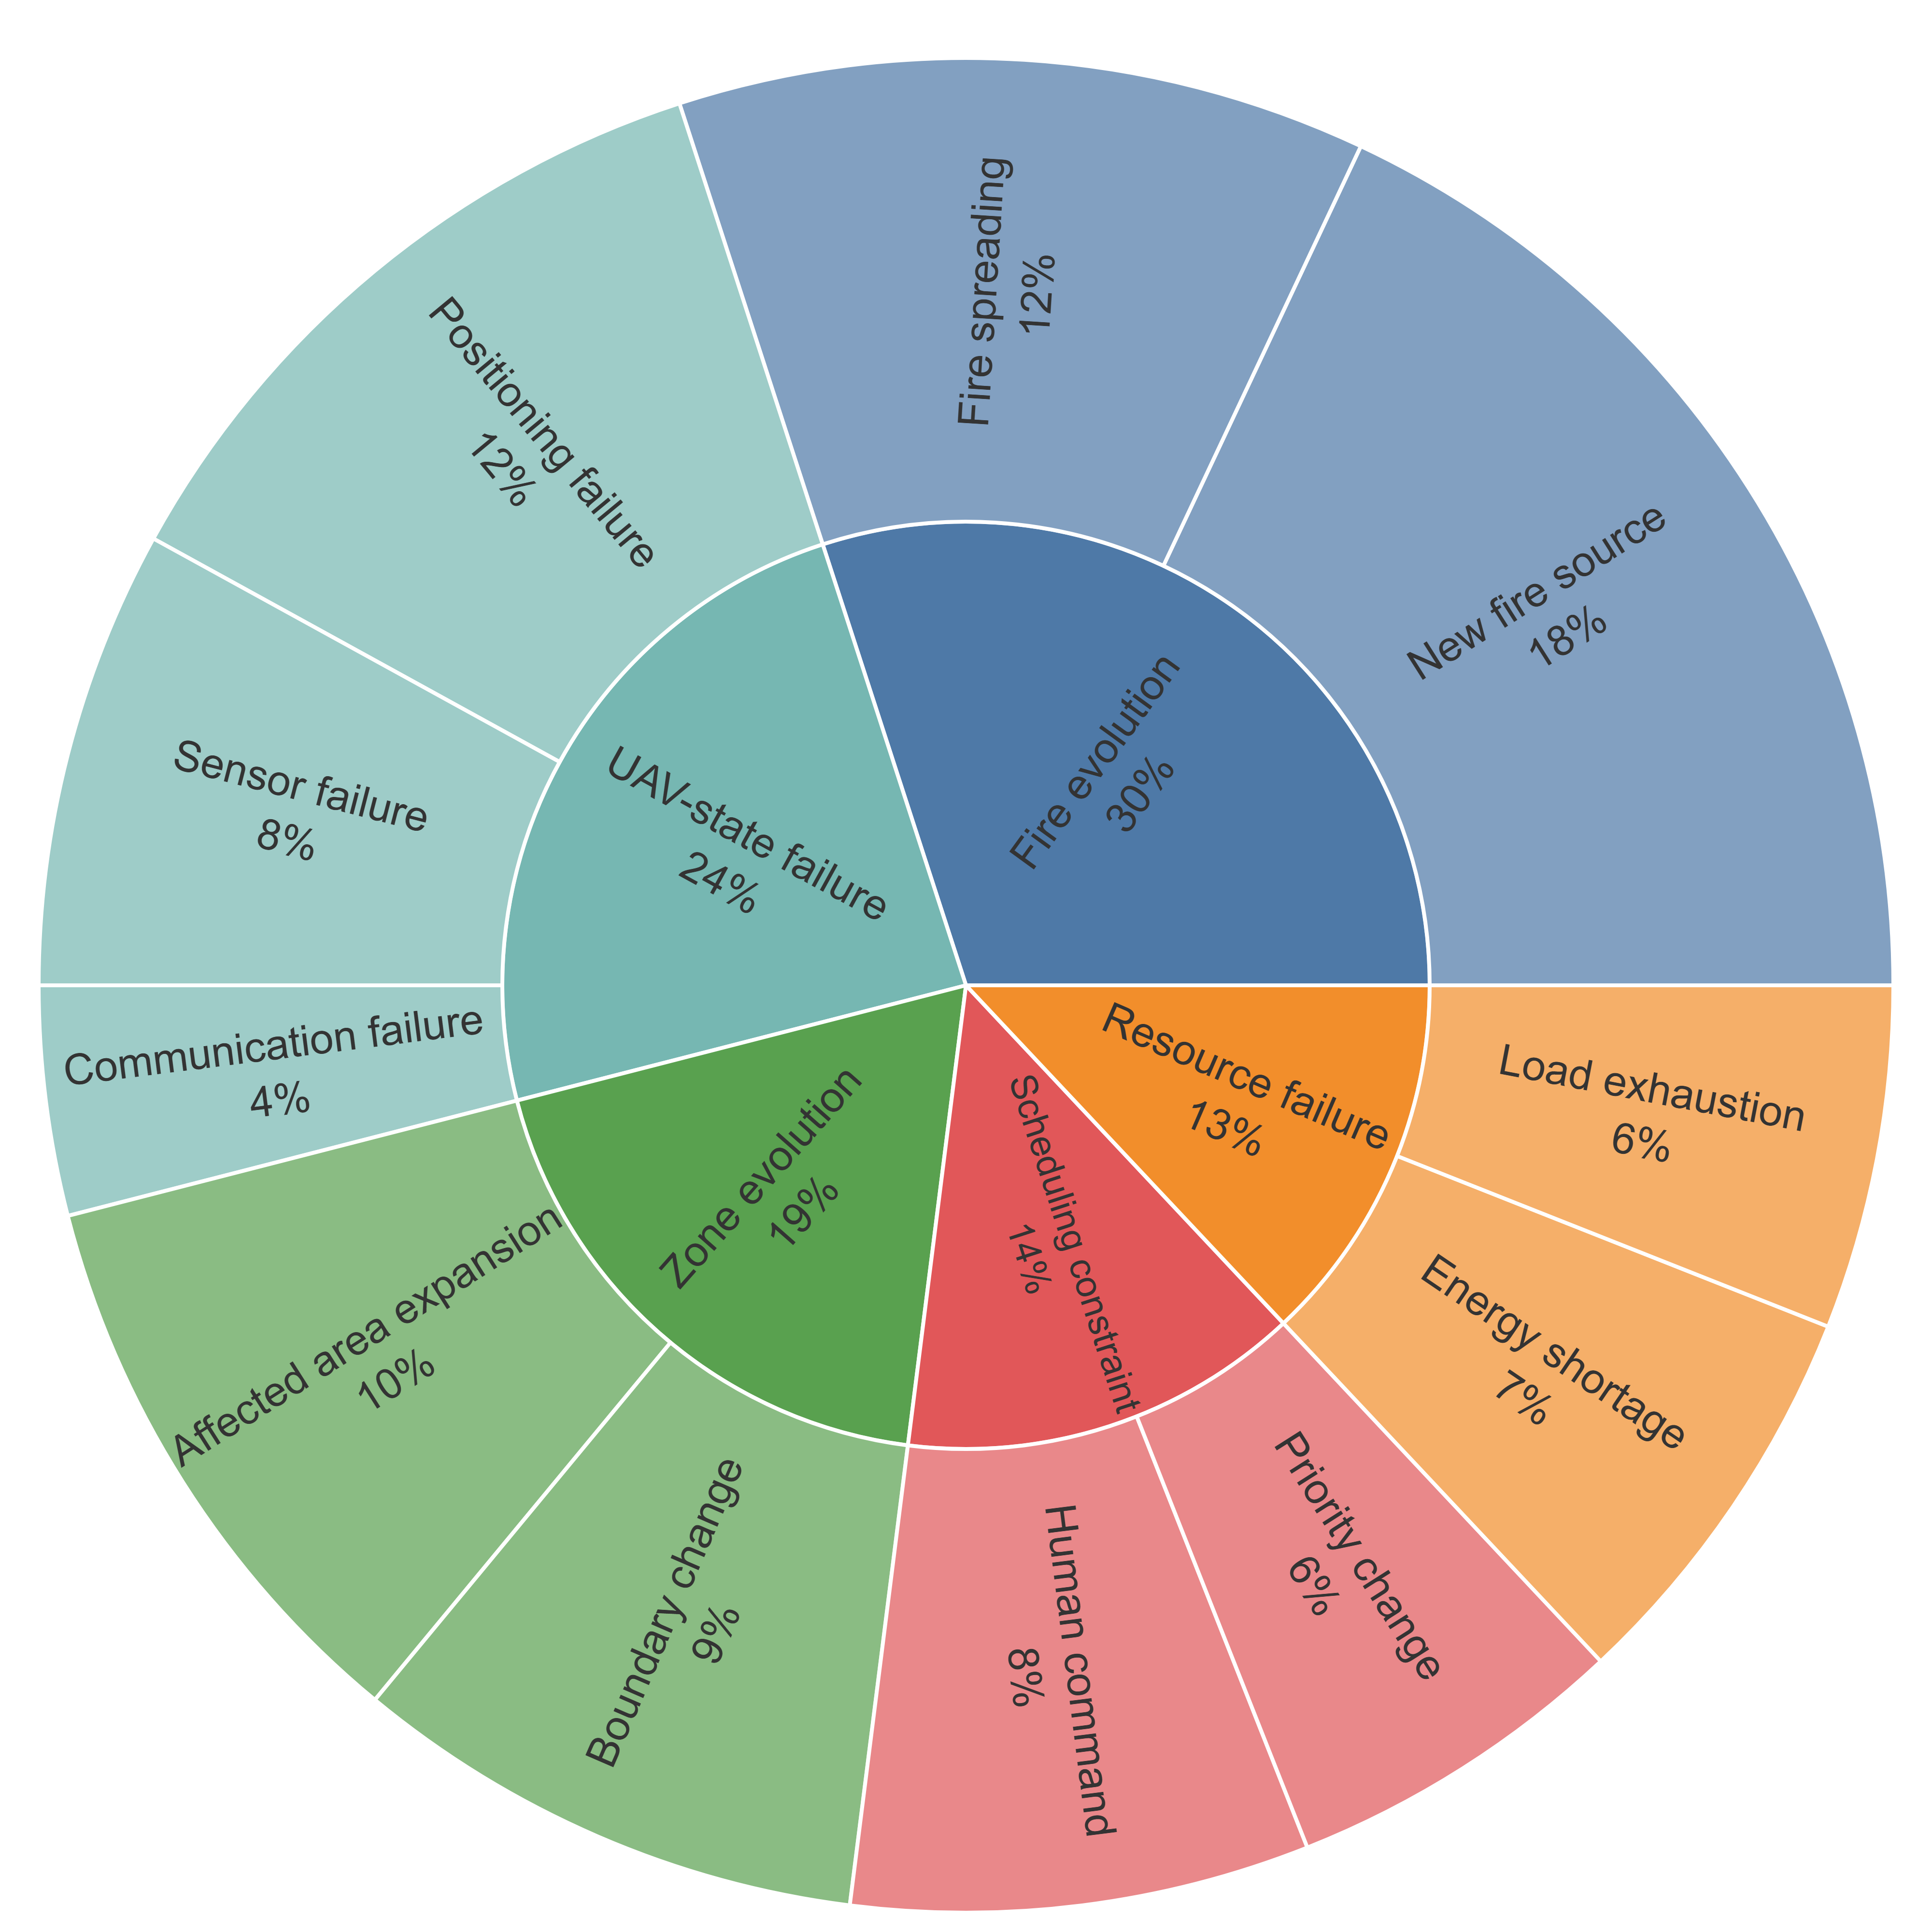
\includegraphics[width=0.35\textwidth]{figures/runtime-perturbation-library.png}}\hspace{0.04\textwidth}
    \subfloat[Distribution of perturbations in hard and expert levels.]{%
        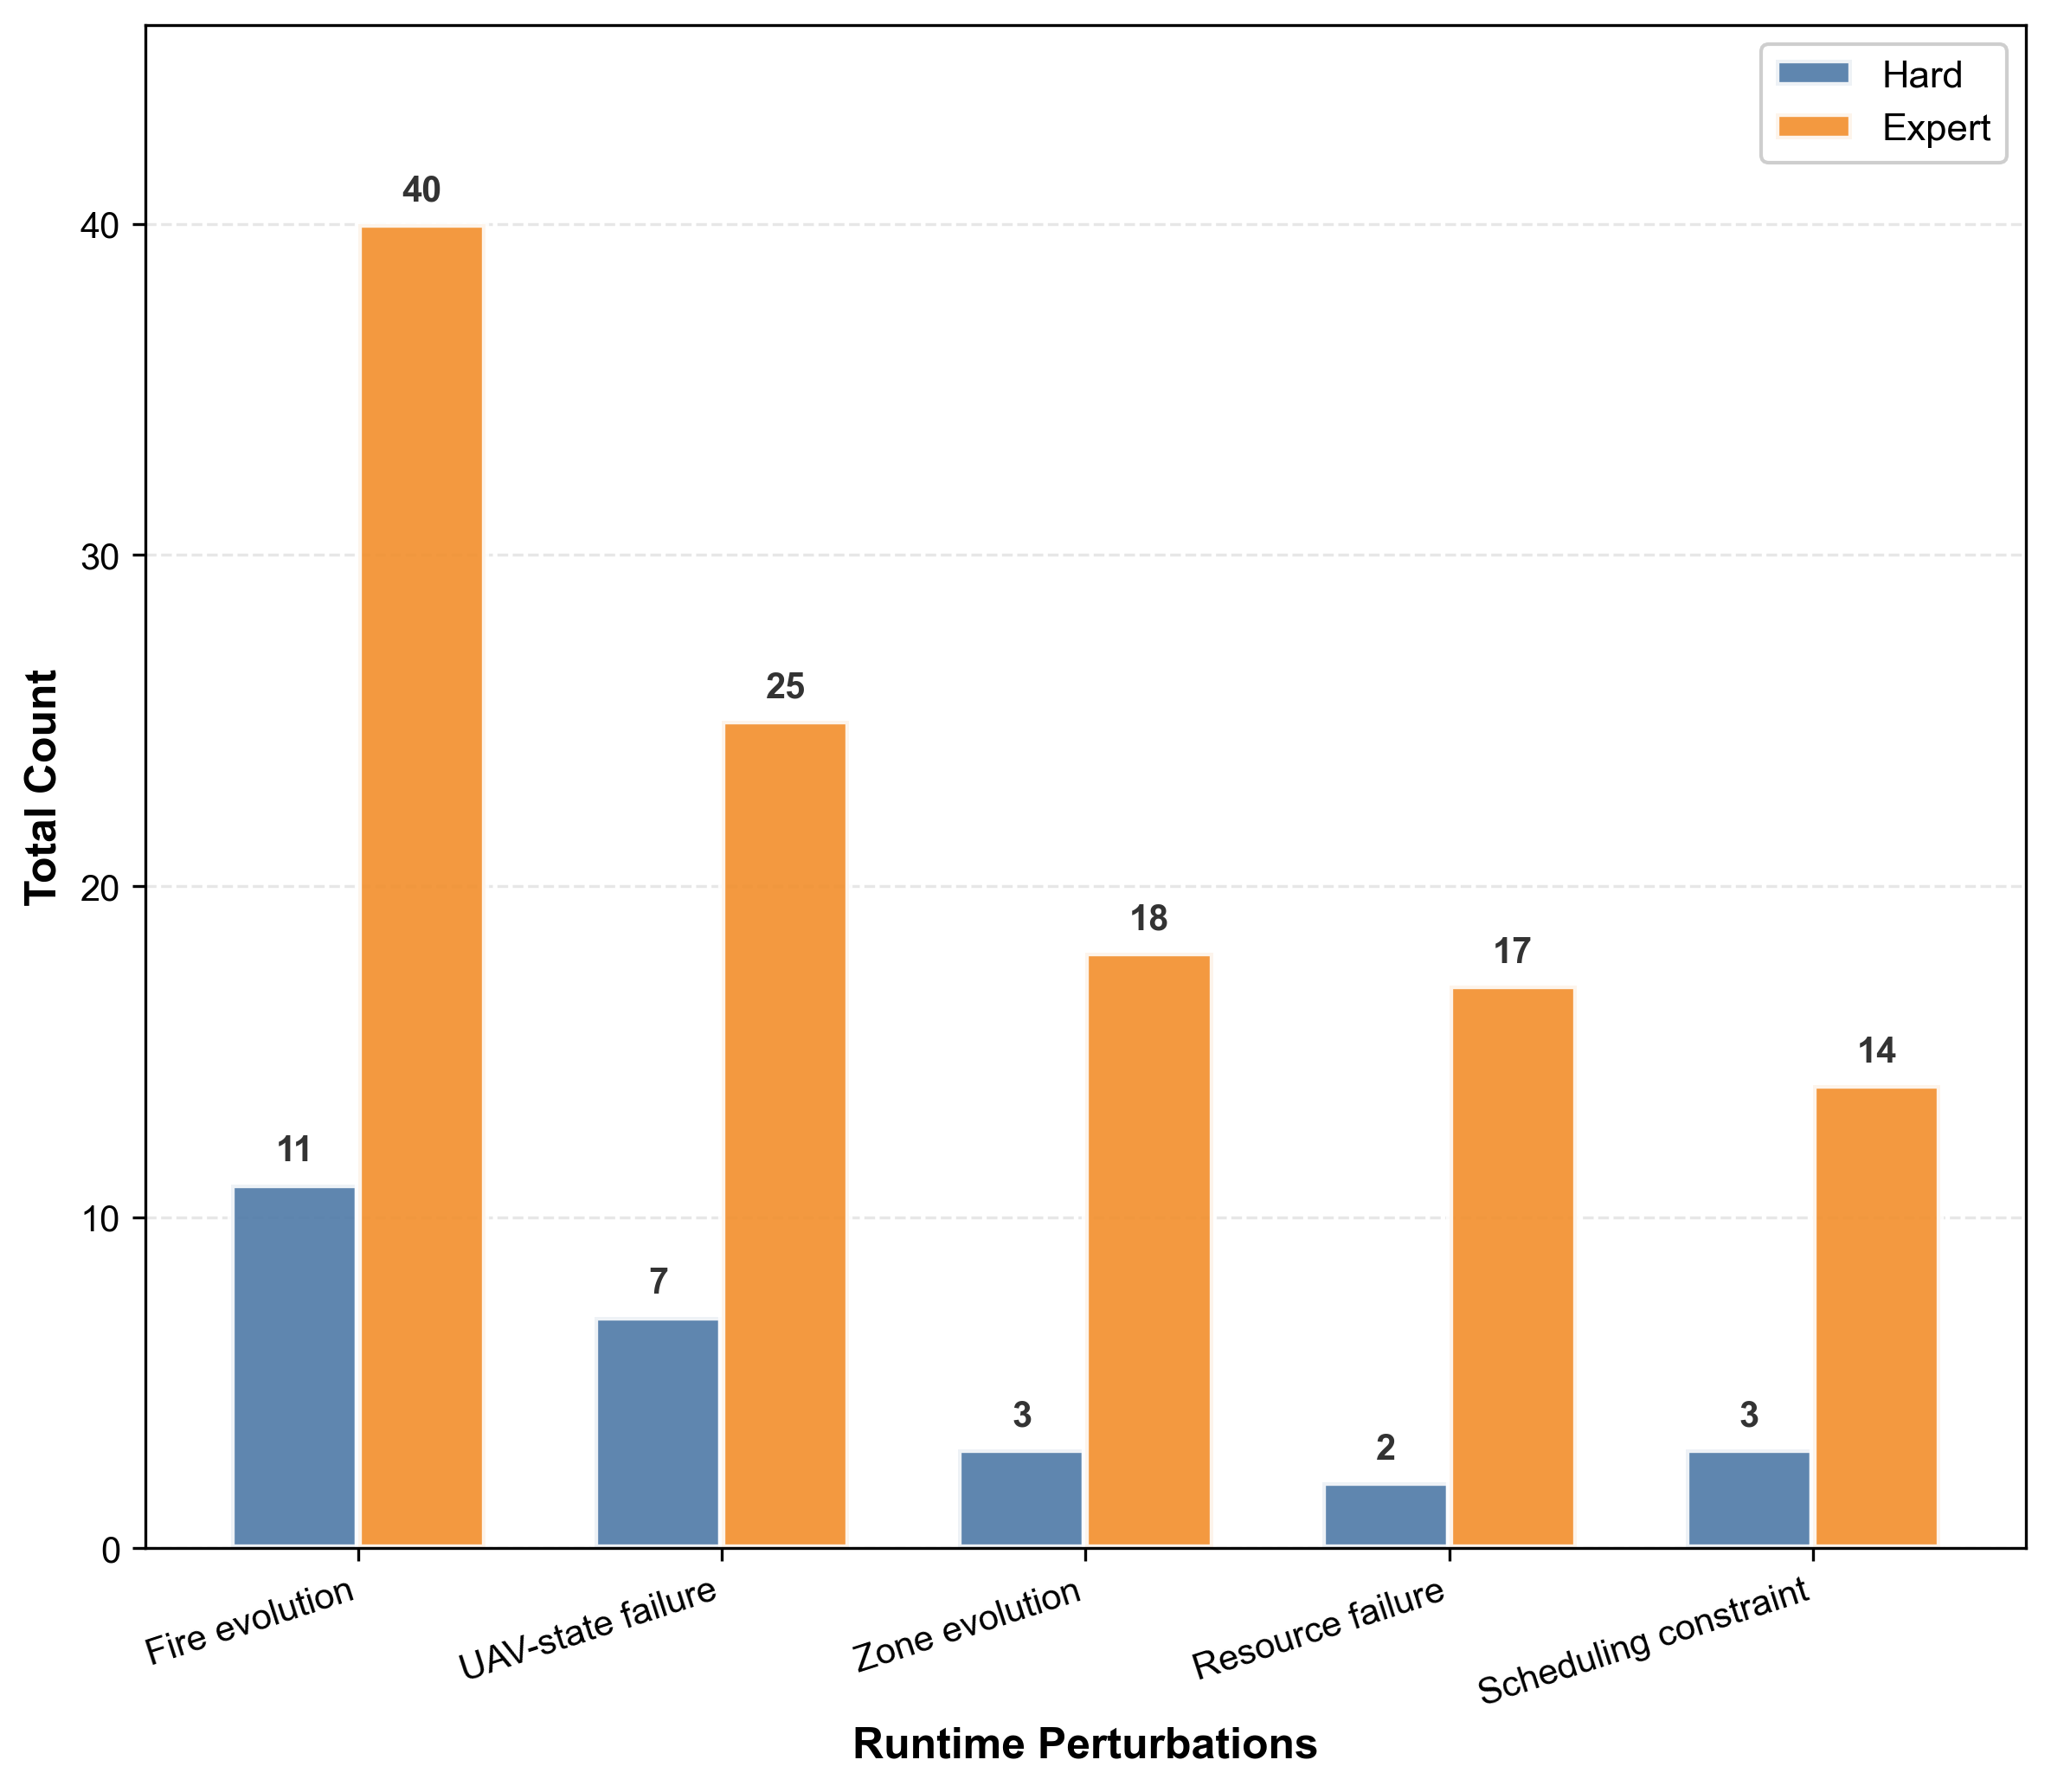
\includegraphics[width=0.35\textwidth]{figures/runtime-perturbation-sampling-distribution.png}}
    \makeatletter
    \long\def\@makecaption#1#2{%
        \@IEEEfigurecaptionsepspace
        \hbox to\hsize{\normalfont\footnotesize\hfil
            \hbox{\normalfont\footnotesize #1.\nobreakspace\nobreakspace #2}\hfil}}
    \makeatother
    \caption{Runtime perturbations used for closed-loop evaluation.}
    \label{fig:runtime-perturbation-distribution}
\end{figure*}

\subsection{Evaluation Metrics}
We evaluate end-to-end behavior using six complementary mission-level metrics:
completion, response, mission time, event stability, resource pressure, and
coordination. They measure objective attainment, response timeliness, execution
efficiency, continuity under perturbations, resource use, and workload balance,
respectively. Event stability is evaluated only in the hard and expert settings,
where runtime perturbations are introduced.

All scores are normalized to $[0,100]$, with higher values indicating better
performance. Let $Z$ be the set of task zones, $c_z\in[0,1]$ the completion
ratio of zone $z$, and $\omega_z$ its priority weight. Let
$\bar t_{\mathrm{resp}}$ and $\tau$ denote the priority-weighted mean time to
first effective intervention and the total mission duration. The six scores are
defined jointly as
\begin{equation}
\begin{aligned}
s_{\mathrm{comp}}
&=100\frac{\sum_{z\in Z}\omega_zc_z}
 {\sum_{z\in Z}\omega_z},\\
s_{\mathrm{resp}}
&=100\left[1-
\left[\frac{\bar t_{\mathrm{resp}}-l_{\mathrm{resp}}}
 {u_{\mathrm{resp}}-l_{\mathrm{resp}}}\right]_0^1\right],\\
s_{\mathrm{time}}
&=100\left[1-
\left[\frac{\tau-l_{\mathrm{time}}}
 {u_{\mathrm{time}}-l_{\mathrm{time}}}\right]_0^1\right],\\
s_{\mathrm{stab}}
&=\frac{100}{N_e}\sum_{e=1}^{N_e}
 \mathbb{I}\bigl(\mathrm{Recovered}(e)\bigr),\\
s_{\mathrm{res}}
 &=100\left[1-\frac{\bar p+\max_jp_j}{2}\right],\\
s_{\mathrm{coord}}
&=100\left[1-
\frac{G(\mathbf{n})+G(\mathbf{d})+G(\boldsymbol{\tau})}{3}\right].
\end{aligned}
\label{eq:mission-level-scores}
\end{equation}
Here, $s_{\mathrm{comp}}$, $s_{\mathrm{resp}}$, $s_{\mathrm{time}}$,
$s_{\mathrm{stab}}$, $s_{\mathrm{res}}$, and $s_{\mathrm{coord}}$ denote the
completion, response, mission time, event stability, resource pressure, and
coordination scores, respectively. $[x]_0^1=\min\{1,\max\{0,x\}\}$ clips a
value $x$ to $[0,1]$;
$l_{\mathrm{resp}}$, $u_{\mathrm{resp}}$, $l_{\mathrm{time}}$, and
$u_{\mathrm{time}}$ are fixed time-reference thresholds. $N_e$ is the number
of runtime perturbations, $e$ indexes these perturbations, and
$\mathrm{Recovered}(e)$ indicates recovery from perturbation $e$ by a feasible
revision within the allowed window. $\mathbb{I}(\cdot)$ is the
indicator function, which equals 1 when its condition is true and 0 otherwise.
$p_j\in[0,1]$ and $\bar p$ denote the resource pressure of UAV $j$ and the
fleet-average resource pressure, respectively, where $j$ indexes the UAVs in
the fleet. $G(\cdot)\in[0,1]$ is the Gini coefficient of the assigned task
counts $\mathbf{n}$, flight distances $\mathbf{d}$, or execution durations
$\boldsymbol{\tau}$.

Because no perturbations are introduced in the simple and normal settings,
their applicable metric set $\mathcal{K}_d$ contains completion, response,
mission time, resource pressure, and coordination; for the hard and expert
settings, it additionally contains event stability.
For each episode $i$ at difficulty level $d$, the score combines the weighted
aggregation of its applicable metrics with a bounded difficulty reward. The
reported score for level $d$ is the mean across its $N_d$ episodes:
\begin{equation}
\begin{aligned}
S_d
&=\frac{1}{N_d}\sum_{i=1}^{N_d}
\left[\sum_{k\in\mathcal{K}_d}w_{k,d}s_{i,k}
\frac{1+\lambda\rho_i}{1+\lambda}\right],\\
w_{k,d}&\geq0,\qquad
\sum_{k\in\mathcal{K}_d}w_{k,d}=1.
\end{aligned}
\label{eq:final-evaluation-score}
\end{equation}
Here, $s_{i,k}$ is the score of episode $i$ for metric $k$, and $w_{k,d}$
is its normalized weight at difficulty level $d$. The coefficient
$\rho_i\in[0,1]$ represents episode difficulty, while $\lambda\geq0$ controls
the difficulty reward; division by $1+\lambda$ keeps $S_d$ within $[0,100]$.
The component scores support diagnostic analysis, whereas $S_d$ provides the
overall comparison score for level $d$.

Together, the staged episode difficulty and decomposed metrics provide a common
basis for testing the three questions examined next: whether CLoMA-UWR sustains
high-level closed-loop decision making, which mechanisms
matter as operational pressure increases, and how much capability for
resource-constrained mission planning can be retained by a compact planner.

\endinput
